\chapter{镜子与薄透镜}\label{ch:b1:mirrors-thin-lenses}

化妆镜中的脸是真实尺寸的两倍大；勺子背面映出的脸又小又正立，
勺子凹面映出的则小而倒立；手持于臂长处的放大镜会把
整个房间倒转过来，凑近时又能放大邮票；一枚小扁豆大小的
手机镜头，能把整条街道映在传感器上。
这些像都服从同一个关于三个距离的代数关系，
本章将建立这一关系——先讨论曲面镜，
再讨论几乎所有光学仪器所用的
薄透镜。

\begin{omfigure}
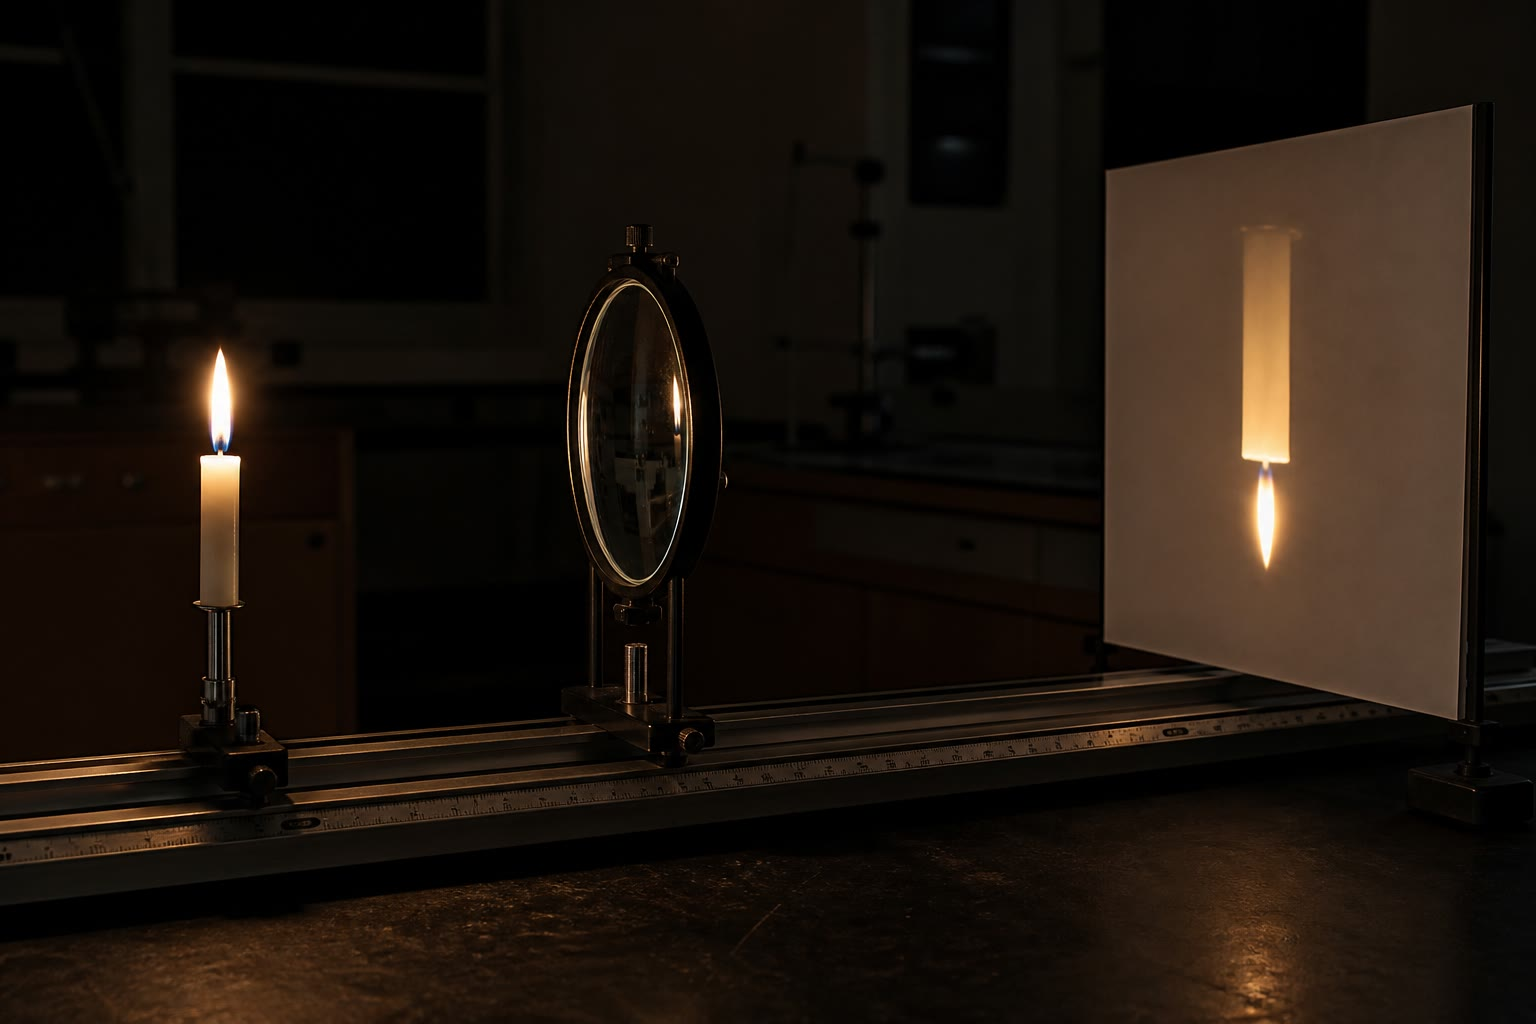
\includegraphics[width=0.60\linewidth]{images/book3/ai/b3-03-lens-candle-image.jpg}

{\small 凸透镜在屏幕上形成烛焰的倒立实像：物距与像距满足本章的共轭关系。}
\end{omfigure}

\section{像与高斯条件}

\begin{definition}[物、像、严格成像]\label{def:b1:mirrors-thin-lenses:image}
\index{像（光学）}\index{物（光学）}\index{严格成像}\index{实像}\index{虚像}
一个光学系统接收来自点 $A$（即\emph{物点}）发出的光线。
若所有出射光线都交于同一点 $A'$，
或其反向延长线都交于同一点 $A'$，则称该系统
对 $A$ 为\emph{严格成像}，$A'$ 即为 $A$ 的\emph{像}。
若出射光线确实相交于 $A'$（可在屏幕上接收到），则称该像为\emph{实像}；
若仅其反向延长线相交（需透过系统观察，
无法投影到屏幕上），则称为\emph{虚像}。类似地，若入射光线从
$A$ 发散，则物为实物；若入射光线会聚于 $A$（位于系统入口之后），
则物为虚物。数对 $(A, A')$ 称为\emph{共轭}的。
\end{definition}

\begin{definition}[共轴系统；高斯条件]\label{def:b1:mirrors-thin-lenses:gauss}
\index{主光轴}\index{高斯条件}\index{近轴光线}
一个\emph{共轴系统}具有一条旋转对称轴，
称为\emph{主光轴}。靠近光轴、与光轴夹小角度的光线，
称为\emph{近轴光线}；仅用近轴光线工作的系统，
称其满足\emph{高斯条件}。在此条件下，
共轴系统对每个点都近似严格成像，
且与光轴垂直的物平面，其对应的像平面也与光轴垂直，
此性质称为\emph{齐明}。
\end{definition}
\admitted

\begin{remark}[为何要求小角度]\label{rem:b1:mirrors-thin-lenses:why}
平面镜是唯一对每个点都严格成像的简单系统。球面镜或透镜
只有在
$\sin\theta \approx \tan\theta \approx \theta$ 的范围内才近似严格成像：
正是这一近似，使斯涅耳定律化为距离之间的线性关系。
超出此范围，点的像便会模糊（\emph{像差}）。
设计者的任务——光阑、
透镜组合、非球面——便是把模糊压低到
眼睛或传感器无法分辨的程度。
\end{remark}

\begin{notation}[代数量与放大率]\label{not:b1:mirrors-thin-lenses:signs}
\index{代数量}\index{横向放大率}
光轴的正方向取入射光的方向；
横向方向取向上。对光轴上的点 $P$、$Q$，
$\overline{PQ}$ 表示代数量（$\overline{PQ} > 0$，
即 $Q$ 位于 $P$ 的下游）；对与光轴垂直的物 $AB$ 与其
像 $A'B'$，\emph{横向放大率}为
\[
\gamma = \frac{\overline{A'B'}}{\overline{AB}} ,
\]
倒立像的放大率为负，
放大像的放大率绝对值大于 $1$。
\end{notation}

\section{球面镜}

\begin{definition}[球面镜]\label{def:b1:mirrors-thin-lenses:mirror}
\index{球面镜}\index{凹面镜}\index{凸面镜}\index{焦点}
\emph{球面镜}是球心为 $C$ 的球冠形反射面，
顶点为 $S$（即其与光轴的交点）。若光线照在凹面一侧（$C$ 位于入射光一侧），
则称为\emph{凹面镜}；否则称为\emph{凸面镜}。其\emph{焦点}
$F$ 是光轴上无穷远点的像；
焦距为 $f = \overline{SF}$。
\end{definition}

\begin{proposition}[球面镜的焦点]\label{prop:b1:mirrors-thin-lenses:focus}
在高斯条件下，焦点为 $SC$ 的中点：
$\overline{SF} = \overline{SC}/2$。凹面镜的 $f < 0$（焦点为实焦点，位于前方）；
凸面镜的 $f > 0$（焦点为虚焦点，位于后方）。
\end{proposition}

\begin{proof}
平行于光轴、高度为 $h$ 的光线射到镜面上的点 $I$，
$I$ 处的法线为半径 $CI$，它与光轴夹角 $\alpha$。
$\sin\alpha = h/R$。光线以与法线相同的角度 $\alpha$ 反射，
反射光线与光轴相交于 $F$，三角形 $CIF$ 中
两角 $\alpha$ 分别在 $C$ 与 $I$ 处，故 $CF = IF$，投影可得
$CF = R/(2\cos\alpha)$。对近轴光线 $\cos\alpha \to 1$，
于是 $CF = R/2$：所有此类光线都与光轴交于同一点，
即 $SC$ 的中点。符号方面，对凹面镜，$C$ 与 $F$ 位于前方
（上游），$\overline{SC} < 0$。
\end{proof}

\begin{theorem}[球面镜的共轭关系]\label{thm:b1:mirrors-thin-lenses:mirrorconj}
\index{共轭关系!球面镜}
在高斯条件下，$A'$ 为光轴上点 $A$ 的像，
满足下列关系：
\[
\frac{1}{\overline{SA'}} + \frac{1}{\overline{SA}} = \frac{2}{\overline{SC}}
= \frac{1}{\overline{SF}},
\qquad
\gamma = -\frac{\overline{SA'}}{\overline{SA}} .
\]
\end{theorem}

\begin{proof}
取一凹面镜，实物 $A$ 位于 $C$ 之外；代数形式
随即涵盖所有情形。从 $A$ 发出的一条光线射到镜面上的 $I$ 点，
高度为 $h$，经反射后与轴交于 $A'$。记 $u$、$u'$、$\omega$
分别为 $AI$、$A'I$、$CI$ 与轴的夹角，近轴时
$u = h/AS$，$u' = h/A'S$，$\omega = h/CS$（均为距离）。由反射定律，
法线 $CI$ 平分 $AI$ 与 $A'I$ 之间的夹角，
即 $\omega - u = u' - \omega$，亦即 $u + u' = 2\omega$，亦即
$1/AS + 1/A'S = 2/CS$；由于 $\overline{SA}$、$\overline{SA'}$、
$\overline{SC}$ 均为负，此即上文所示关系。关于放大率，
光线 $B \to S \to B'$ 在顶点处反射，
与轴夹角相等：按长度计 $A'B'/SA' = AB/SA$，且像
是倒立的，$\gamma = -\overline{SA'}/\overline{SA}$。
\end{proof}

\begin{method}[在镜中作像]\label{met:b1:mirrors-thin-lenses:mirrorrays}
对轴外物点 $B$，作出四条特殊光线中的两条，
其交点（或其延长线的交点）即为 $B'$：
\begin{enumerate}
  \item 平行于轴 $\to$ 经 $F$ 反射；
  \item 经 $F$ $\to$ 平行于轴反射；
  \item 经 $C$ $\to$ 沿原路反射；
  \item 射向顶点 $S$ $\to$ 关于轴对称反射。
\end{enumerate}
于是 $A'$ 为由 $B'$ 向轴所作垂线的垂足。
\end{method}

\begin{omfigure}
\begin{tikzpicture}[font=\small, x=1cm, y=1cm]
  % concave mirror, S at (0,0), C at (-4,0), F at (-2,0); object A at (-6,0) height 1
  \draw[-Stealth] (-7.5,0) -- (1.0,0);
  \draw[thick, omDef] (-4,0) ++(-20:4) arc (-20:20:4);
  \foreach \x/\n in {0/S, -4/C, -2/F} {\fill (\x,0) circle (1.3pt); \node[below] at (\x,-0.05) {$\n$};}
  % object AB at x=-6, h=1.0 ; image: 1/SA' = 1/SF - 1/SA = -1/2 + 1/6 = -1/3 -> SA'=-3, gamma=-0.5
  \draw[-Stealth, very thick, omThm] (-6,0) -- (-6,1.0); \node[above] at (-6,1.0) {$B$}; \node[below] at (-6,-0.05) {$A$};
  \draw[-Stealth, very thick, omThm] (-3,0) -- (-3,-0.5); \node[below] at (-3,-0.5) {$B'$}; \node[above] at (-3,0.05) {$A'$};
  % ray 1: parallel from B to mirror at height 1 (mirror x approx -0.126), then through F
  \draw[omProp] (-6,1.0) -- (-0.13,1.0);
  \draw[omProp, -Stealth] (-0.13,1.0) -- (-3,-0.5);
  \draw[omProp] (-3,-0.5) -- (-4.5,-1.28);
  % ray 2: from B through C to mirror, reflected back on itself: line B(-6,1) C(-4,0): slope -0.5, hits mirror near x=-0.06,y=-1.97? too far; use ray through F instead:
  % ray 3: from B through F(-2,0): slope = -1/4; hits mirror at y = (x+2)*(-1/4) at x≈-0.07: y=-0.48 -> reflected parallel to axis at y=-0.48? Wait image height is -0.5 -> parallel ray at y=-0.5 passes B'. good
  \draw[omExo] (-6,1.0) -- (-0.03,-0.5);
  \draw[omExo, -Stealth] (-0.03,-0.5) -- (-3,-0.5);
  \draw[omExo] (-3,-0.5) -- (-4.5,-0.5);
\end{tikzpicture}

{\small 凹面镜（$C$ 为曲率中心，焦点 $F$ 位于半径中点）。对于
物体 $AB$ 位于 $C$ 之外时，平行于轴的光线经反射后过 $F$，
过 $F$ 的光线经反射后平行于轴：二者相交于 $B'$——一个实像，
倒立、缩小，位于 $F$ 与 $C$ 之间。}
\end{omfigure}

\begin{example}[剃须镜与后视镜]\label{ex:b1:mirrors-thin-lenses:mirrors}
一面曲率半径为 \qty{60}{cm}（$f = \qty{-30}{cm}$）的凹面镜，镜前
\qty{20}{cm} 处有一张人脸：$1/\overline{SA'} = -1/30 + 1/20 = 1/60$，
$\overline{SA'} = \qty{+60}{cm}$——位于镜后，为虚像——
且 $\gamma = -60/(-20) = +3$：正立、放大三倍，这就是
剃须镜。一面曲率半径为 \qty{2.0}{m}（$f = \qty{+1.0}{m}$）的凸面镜，
其后 \qty{20}{m} 处有一辆汽车：$1/\overline{SA'} = 1 + 1/20$，
$\overline{SA'} = \qty{0.95}{m}$（虚像，位于镜后），$\gamma = +0.048$：
正立、缩小二十倍，因而视场宽阔——即
后视镜，镜上的警示语为“物体
比看上去更近”。
\end{example}

\section{薄透镜}

\begin{definition}[薄透镜]\label{def:b1:mirrors-thin-lenses:lens}
\index{薄透镜}\index{凸透镜}\index{凹透镜}\index{光心}\index{焦距}\index{光焦度}
由两个球面（或平面）所界的透明介质称为\emph{透镜}；
当其厚度相对于曲率半径及所涉距离可忽略时，称之为\emph{薄}透镜，
以致两个顶点
合为一点，即\emph{光心} $O$。过 $O$ 的光线
不发生偏折。\emph{像方焦点} $F'$ 是
轴上无穷远点的像；\emph{物方焦点} $F$ 是
像位于无穷远的点；二者到
$O$ 的距离相等，$\overline{OF'} = -\overline{OF} = f'$，称为\emph{焦距}。
透镜在 $f' > 0$ 时为\emph{凸透镜}（$F'$ 为实焦点，位于下游；
边缘比中心薄），$f' < 0$ 时为\emph{凹透镜}。其\emph{光焦度}
$V = 1/f'$ 以\emph{屈光度}为单位度量
（$\qty{1}{\delta} = \qty{1}{m^{-1}}$）。
\end{definition}

\begin{theorem}[薄透镜的共轭关系]\label{thm:b1:mirrors-thin-lenses:lensconj}
\index{共轭关系!薄透镜}\index{笛卡儿关系}\index{牛顿关系}
在高斯条件下，$A'$ 为轴上点 $A$ 的像，
满足笛卡儿关系：
\[
\frac{1}{\overline{OA'}} - \frac{1}{\overline{OA}} = \frac{1}{f'},
\qquad
\gamma = \frac{\overline{OA'}}{\overline{OA}},
\]
亦等价地满足牛顿关系：
\[
\overline{FA}\cdot\overline{F'A'} = -f'^2,
\qquad
\gamma = \frac{f'}{\overline{FA}} = -\frac{\overline{F'A'}}{f'} .
\]
\end{theorem}

\begin{proof}[部分证明]
关键事实是，薄透镜使穿过它、高度为
$h$ 的光线向轴偏折 $h/f'$ 角，无论光线方向如何
——透镜的每个区域都相当于一个薄棱镜（见\cref{rem:b1:rays-reflection-refraction:thin}）
其顶角对球面而言随 $h$ 线性增长；此线性关系
对近轴光线严格成立，在本阶段不加证明地承认，
其由两个球面上的斯涅耳定律推出（见本科二年级分册）。承认此点后，
从 $A$ 发出的光线（距离 $p = -\overline{OA} > 0$，对实物而言）
到达高度为 $h$ 的透镜处时斜率为 $h/p$，
经偏折 $h/f'$ 后，出射斜率为 $h/p - h/f'$；该光线与轴交于
$A'$，且 $h/\overline{OA'} = h/f' - h/p$，即 $1/\overline{OA'}
- 1/\overline{OA} = 1/f'$，与 $h$ 无关：从 $A$ 发出的所有光线会聚于
$A'$。过中心的光线 $B \to O \to B'$ 为直线，故
$\overline{A'B'}/\overline{AB} = \overline{OA'}/\overline{OA}$。牛顿
形式可由代换 $\overline{OA} = \overline{OF} + \overline{FA}
= -f' + \overline{FA}$ 及 $\overline{OA'} = f' + \overline{F'A'}$ 得出。
\end{proof}

\begin{method}[由薄透镜作像]\label{met:b1:mirrors-thin-lenses:lensrays}
由 $B$ 发出的三条特殊光线：
\begin{enumerate}
  \item 过 $O$：方向不变；
  \item 平行于主轴：出射后过 $F'$；
  \item 过 $F$：出射后平行于主轴。
\end{enumerate}
任取两条即可；对于凹透镜，使用其延长线（射向
透镜后方 $F$ 的光线出射后平行于主轴；平行光线出射后如同从
前方 $F'$ 发出）。
\end{method}

\begin{omfigure}
\begin{tikzpicture}[font=\small, x=1cm, y=1cm]
  % converging lens f'=2 at O=(0,0); object at OA=-3, h=1 -> 1/OA' = 1/2 - 1/3 = 1/6 -> OA'=6, gamma=-2
  \draw[-Stealth] (-4.3,0) -- (7.0,0);
  \draw[very thick, omDef, Stealth-Stealth] (0,-1.9) -- (0,1.9);
  \foreach \x/\n in {0/O, -2/F, 2/F'} {\fill (\x,0) circle (1.3pt); \node[below] at (\x,-0.05) {$\n$};}
  \draw[-Stealth, very thick, omThm] (-3,0) -- (-3,0.9); \node[above] at (-3,0.9) {$B$}; \node[below] at (-3,-0.05) {$A$};
  \draw[-Stealth, very thick, omThm] (6,0) -- (6,-1.8); \node[below] at (6,-1.8) {$B'$}; \node[above] at (6,0.05) {$A'$};
  \draw[omProp] (-3,0.9) -- (0,0.9) -- (6,-1.8);
  \draw[omExo] (-3,0.9) -- (6,-1.8);
  \draw[omThm!70] (-3,0.9) -- (0,-0.9) -- (6,-0.9);
  \node[omDef] at (0.55,1.75) {$L$};
\end{tikzpicture}

{\small 凸透镜：物 $AB$ 位于 $F$ 之外。过 $O$ 的光线直行，
平行光线经 $F'$ 折射，过 $F$ 的光线出射后平行于主轴，
三条光线交于 $B'$：实像，倒立。此处
$\overline{OA} = -1.5f'$，故 $\overline{OA'} = 3f'$，$\gamma = -2$。}
\end{omfigure}

\begin{omfigure}
\begin{tikzpicture}[font=\small, x=1cm, y=1cm]
  % diverging lens f'=-2 at O; object at OA=-3, h=1.2 -> 1/OA' = -1/2 - 1/3 = -5/6 -> OA' = -1.2, gamma = 0.4
  \draw[-Stealth] (-4.3,0) -- (4.5,0);
  \draw[very thick, omDef, Stealth-Stealth] (0,-1.9) -- (0,1.9);
  \foreach \x/\n in {0/O, 2/F, -2/F'} {\fill (\x,0) circle (1.3pt); \node[below] at (\x,-0.05) {$\n$};}
  \draw[-Stealth, very thick, omThm] (-3,0) -- (-3,1.2); \node[above] at (-3,1.2) {$B$}; \node[below] at (-3,-0.05) {$A$};
  \draw[-Stealth, very thick, omThm] (-1.2,0) -- (-1.2,0.48); \node[above] at (-1.2,0.5) {$B'$}; \node[below] at (-1.2,-0.05) {$A'$};
  \draw[omProp] (-3,1.2) -- (0,1.2) -- (4.0,3.6*1.2/1.8+0) ;
  \draw[omProp, dashed] (0,1.2) -- (-2,0);
  \draw[omExo] (-3,1.2) -- (0,0) -- (4.0,-1.6);
  \draw[omExo, dashed] (-1.2,0.48) -- (0,0);
  \node[omDef] at (0.55,1.75) {$L$};
\end{tikzpicture}

{\small 凹透镜（$F'$ 在前方，$F$ 在后方）：平行光线出射后如同从
$F'$ 发出，过中心的光线直行；二者的反向延长线交于 $B'$，
得到虚像：正立、缩小，
且与物的位置无关。}
\end{omfigure}

\begin{example}[同一透镜的三种用法]\label{ex:b1:mirrors-thin-lenses:lensuses}
凸透镜，$f' = \qty{5.0}{cm}$。印章置于 \qty{3.0}{cm} 处：
$1/\overline{OA'} = 1/5 - 1/3 = -2/15$，$\overline{OA'} = \qty{-7.5}{cm}$，
虚像，$\gamma = +2.5$：放大镜。灯置于 \qty{20}{cm} 处：
$\overline{OA'} = \qty{6.7}{cm}$，实像，$\gamma = -1/3$：缩小的
倒立像落在卡片上。窗户位于 \qty{4}{m} 远处：$\overline{OA'}
\approx f'$，焦平面上得到微小的倒立像——照相机。
三种用法，同一关系。
\end{example}

\begin{proposition}[纵向放大率]\label{prop:b1:mirrors-thin-lenses:longitudinal}
\index{纵向放大率}
若物沿主轴移动 $\dd\overline{OA}$，则像
移动 $\dd\overline{OA'} = \gamma^2\,\dd\overline{OA}$，
方向相同。
\end{proposition}

\begin{proof}
在 $f'$ 固定时对笛卡儿关系求微分：
$-\dd\overline{OA'}/\overline{OA'}^2 + \dd\overline{OA}/\overline{OA}^2 = 0$,
故 $\dd\overline{OA'} = (\overline{OA'}/\overline{OA})^2\,\dd\overline{OA}$。
\end{proof}

\begin{remark}[焦深]\label{rem:b1:mirrors-thin-lenses:depth}
投影仪的 $\gamma = -50$，$\gamma^2 = 2500$：一张幻灯片
在灯的热量作用下弯曲 \qty{0.1}{mm}，其像
便偏离屏幕平面 \qty{25}{cm}。反之，照相机（$\abs\gamma
\ll 1$）允许物有较大位移，而像仅产生微小移动——
此即景深。
\end{remark}

\section{焦距的测量}

\begin{method}[自准直法]\label{met:b1:mirrors-thin-lenses:autocollimation}
\index{自准直法}
将平面镜紧贴放在透镜后方，沿主轴移动一个被照亮的物（毛玻璃上的
十字），直到其经透镜后被镜面反射回来所成的像
清晰地落在物本身上，且倒立、大小相同。
此时物位于焦平面上：光线离开透镜时平行，
经镜面返回后仍平行，并在焦平面上重新会聚。
物与透镜的距离为 $f'$。
\end{method}

\begin{proposition}[贝塞尔法]\label{prop:b1:mirrors-thin-lenses:bessel}
\index{贝塞尔法}\index{西尔伯曼法}
物与屏相距 $D$ 固定。凸透镜
在屏上形成清晰实像的位置：当 $D > 4f'$ 时恰有两个，
当 $D = 4f'$ 时有一个，当 $D < 4f'$ 时则无。两位置
相距 $d$，且
\[
f' = \frac{D^2 - d^2}{4D} .
\]
当 $D = 4f'$（西尔伯曼法）时，唯一位置给出 $\gamma = -1$。
\end{proposition}

\begin{proof}
设 $p = -\overline{OA} > 0$ 为物与透镜的距离；则
$\overline{OA'} = D - p$，由笛卡儿关系得 $1/(D - p) + 1/p = 1/f'$，
即 $p^2 - Dp + Df' = 0$：判别式为 $D^2 - 4Df'$，当且仅当
$D > 4f'$ 时为正。两根 $p_{1,2} = (D \mp \sqrt{D^2 - 4Df'})/2$ 之和为
$D$（两位置对称：物距与像距互换），
二者之差为 $d = \sqrt{D^2 - 4Df'}$，由此解出 $f'$。当
$D = 4f'$ 时，$p = 2f' = \overline{OA'}$，且 $\gamma = -1$。
\end{proof}

\begin{omfigure}
\begin{tikzpicture}[font=\small, x=1cm, y=1cm]
  % D = 8 (units), f'=1.5 -> d = sqrt(64-48)=4 ; positions p = 2 and 6
  \draw[-Stealth] (-0.8,0) -- (8.8,0);
  \draw[very thick, omThm, -Stealth] (0,0) -- (0,0.5); \node[left] at (0,0.3) {物};
  \draw[very thick] (8,-1.6) -- (8,1.6); \node[right] at (8,1.3) {屏幕};
  \draw[very thick, omDef, Stealth-Stealth] (2,-1.4) -- (2,1.4); \node[omDef, above] at (2,1.45) {$L$（位置 1）};
  \draw[very thick, omDef!45, Stealth-Stealth] (6,-1.4) -- (6,1.4); \node[omDef!60!black, above] at (6,1.45) {$L$（位置 2）};
  % position 1: p=2, image at 6 from lens -> gamma=-3: image height -2.4 at x=8
  \draw[omProp] (0,0.5) -- (2,0.5) -- (8,-1.5);
  \draw[omProp] (0,0.5) -- (8,-1.5);
  \draw[-Stealth, very thick, omThm] (8,0) -- (8,-1.5);
  % position 2: p=6, image at 2 -> gamma=-1/3: height -0.267
  \draw[omExo!80, dashed] (0,0.5) -- (6,0.5) -- (8,-0.167);
  \draw[Stealth-Stealth] (0,-1.9) -- (8,-1.9) node[midway, below] {$D$};
  \draw[Stealth-Stealth] (2,-1.0) -- (6,-1.0) node[midway, below] {$d$};
\end{tikzpicture}

{\small 贝塞尔方法：物与屏幕固定于 $D > 4f'$ 处；透镜
在两个相距 $d$ 的对称位置上给出清晰的像
（一次放大、一次缩小），且 $f' = (D^2 - d^2)/4D$。}
\end{omfigure}

\section{两个薄透镜}

\begin{proposition}[接触的透镜；无焦双透镜]\label{prop:b1:mirrors-thin-lenses:doublet}
\index{无焦系统}\index{角放大率}
两个薄透镜紧贴时，等效于一个光焦度为
$V = V_1 + V_2$ 的薄透镜。两透镜的放置满足 $F_1' = F_2$ 时，构成一个
\emph{无焦}系统：平行光束出射后仍为平行光束，而
与光轴成夹角 $\alpha$ 的光束出射后夹角为 $\alpha' = G\alpha$，其中
\emph{角放大率} $G = -f_1'/f_2'$。
\end{proposition}

\begin{proof}
像 $A_1$ 由 $L_1$ 所成，即为 $L_2$ 的物。紧贴时，
$O_1 = O_2 = O$，故 $1/\overline{OA_1} - 1/\overline{OA} = V_1$，且
$1/\overline{OA'} - 1/\overline{OA_1} = V_2$；两式相加。对于无焦系统，
以角度 $\alpha$ 入射的平行光束在公共焦平面上会聚，
离轴高度为 $h = f_1'\alpha$（经过 $O_1$ 的光线）；从 $L_2$ 看去，该点
位于其物方焦平面上，故光束出射后仍平行，
其方向由经该点穿过 $O_2$ 的光线的倾角决定，即 $\alpha' = -h/f_2'$。
\end{proof}

\begin{example}[一行式望远镜]\label{ex:b1:mirrors-thin-lenses:afocal}
$f_1' = \qty{1000}{mm}$，$f_2' = \qty{25}{mm}$，$G = -40$；月球，
视宽半度，变为 $20^\circ$ 的圆盘——即下一章中的天文
望远镜。若目镜为凹透镜，
$f_2' = \qty{-25}{mm}$，$G = +40$：正立的像，即伽利略望远镜。
\end{example}

\section{练习}

\begin{exercise}[$\star$]\label{exo:b1:mirrors-thin-lenses:1}
一凹面镜，其曲率半径 $R = \qty{40}{cm}$。求放在
距顶点 \qty{60}{cm}、\qty{30}{cm} 和 \qty{10}{cm} 处的物体的像：
位置、虚实及放大率。
\end{exercise}

\begin{exercise}[$\star$]\label{exo:b1:mirrors-thin-lenses:2}
一凸透镜的焦距 $f' = \qty{5.0}{cm}$。求物体
分别位于距透镜 \qty{20}{cm} 和 \qty{3.0}{cm} 处时的像，并画出作图。
\end{exercise}

\begin{exercise}[$\star$]\label{exo:b1:mirrors-thin-lenses:3}
求焦距为 \qty{25}{cm} 的透镜的光焦度；
求光焦度为 \qty{-2.0}{\delta} 的透镜的焦距；求
光焦度分别为 \qty{+3.0}{\delta} 与 \qty{-1.0}{\delta} 的两透镜紧贴时的焦距。
\end{exercise}

\begin{exercise}[$\star$]\label{exo:b1:mirrors-thin-lenses:4}
已知 $f' = \qty{10}{cm}$，物体位于 $F$ 前 \qty{15}{cm} 处，
用牛顿关系式求像的位置和 $\gamma$，并用
笛卡儿关系式检验。
\end{exercise}

\begin{exercise}[$\star\star$]\label{exo:b1:mirrors-thin-lenses:5}
一凸面后视镜，曲率半径 $R = \qty{2.0}{m}$。一辆
高 \qty{1.5}{m} 的汽车位于镜后 \qty{20}{m} 处：求像的位置及像高，
并解释警示语“镜中物体比看上去更近”。
\end{exercise}

\begin{exercise}[$\star\star$]\label{exo:b1:mirrors-thin-lenses:6}
一照相机镜头，$f' = \qty{50}{mm}$，对焦于
距离为 \qty{2.0}{m} 的被摄物体。镜头须从无穷远位置移动多少？
放大率为多少？摄影者须后退多远，才能使
身高 \qty{1.8}{m} 的人恰好充满传感器 \qty{24}{mm} 的高度？
\end{exercise}

\begin{exercise}[$\star\star$]\label{exo:b1:mirrors-thin-lenses:7}
一投影仪须将宽 \qty{36}{mm} 的幻灯片投射为宽 \qty{1.8}{m} 的
画面，屏幕距透镜 \qty{5.0}{m}。求所需的焦距
及幻灯片–透镜距离。为何幻灯片要
倒插放置？
\end{exercise}

\begin{exercise}[$\star\star$]\label{exo:b1:mirrors-thin-lenses:8}
用光线图说明，为何自准直能准确定出焦平面，
以及为何返回的像倒立且与物等大。
若将镜面稍稍倾斜，
返回的像会如何变化？
\end{exercise}

\begin{exercise}[$\star\star$]\label{exo:b1:mirrors-thin-lenses:9}
物与屏幕相距 \qty{1.00}{m}，在
透镜处于两个相距 \qty{40}{cm} 的位置时均可得清晰的像。求 $f'$。
该透镜仍能投射清晰像的最短物–屏距离为多少，
以及此时的放大率为多少？
\end{exercise}

\begin{exercise}[$\star\star\star$]\label{exo:b1:mirrors-thin-lenses:10}
凸透镜 $L_1$（$f_1' = \qty{20}{cm}$）之后相距 \qty{15}{cm}
处再置一凹透镜 $L_2$（$f_2' = \qty{-10}{cm}$）。求
无穷远物体所成像的位置。证明：视角为
$\alpha$ 的远处物体，其像高为 $\qty{40}{cm}\times\alpha$，并
将此值与该组合的长度相比较，
说明长焦镜头的原理。
\end{exercise}

\begin{exercise}[$\star\star\star$]\label{exo:b1:mirrors-thin-lenses:11}
一凹面镜在距灯丝 \qty{80}{cm} 的屏幕上成灯丝的像，
像的大小为灯丝的三倍。求
镜子的位置及其曲率半径。
\end{exercise}

\begin{exercise}[$\star\star\star$]\label{exo:b1:mirrors-thin-lenses:12}
太阳的视角为 $0.53^\circ$。一直径为
\qty{10}{cm}、焦距为 \qty{50}{cm} 的凸透镜将太阳成像于一张纸上。
求像的直径、透镜所收集的功率（太阳辐照度为
\qty{1.0}{kW/m^2}），以及像处的辐照度；将其与太阳直射辐照度相比较，
并给出结论。
\end{exercise}

\section{问题：幻灯投影仪}

\begin{problem}[{周末问题——一片透镜，在光具座上测量，
然后要求将一张 35 毫米幻灯片投过整个大厅：投影仪如何设计、
调焦，并配上长距离转换器}]
\label{pb:b1:mirrors-thin-lenses:1}
投影镜头 $L_1$ 为一焦距 $f_1'$ 未知的薄凸透镜。
幻灯片高 \qty{24}{mm}，宽 \qty{36}{mm}。

\medskip
\noindent\textbf{第一部分——光具座上的透镜。}
\begin{enumerate}
  \item 写出薄透镜的笛卡儿关系式及其放大率，
        并说明符号约定。
  \item 物与屏幕之间的距离固定为 $D$。证明：
        屏幕上要得到实像，须满足 $D \geq 4f_1'$。
  \item 证明：当 $D > 4f_1'$ 时，能得到清晰像的两个透镜位置
        关于物与屏幕的中点对称，
        并证明 $f_1' = (D^2 - d^2)/4D$，其中 $d$
        为两位置之间的距离。
  \item 取 $D = \qty{80.0}{cm}$，$d = \qty{40.0}{cm}$，计算
        $f_1'$。
  \item 透镜装在一厚的镜筒中，其光心无法精确确定，
        为何这不影响该方法？
  \item 距离的不确定度分别为 $u(D) = \qty{0.2}{cm}$ 和
        $u(d) = \qty{0.5}{cm}$。计算 $u(f_1')$，并写出结果。
  \item 求两个位置各自的放大率，
        哪一个对应投影仪？
  \item 求能得到清晰像的最小 $D$，
        以及此时的放大率（西尔伯曼）。
\end{enumerate}

\medskip
\noindent\textbf{第二部分——投射画面。}
屏幕上的画面宽须为 \qty{1.80}{m}。取
$f_1' = \qty{15.0}{cm}$。
\begin{enumerate}[resume]
  \item 所需的放大率为多少（含符号）？
  \item 计算透镜与屏幕的距离，以及幻灯片与透镜的距离。
  \item 为何幻灯片要倒插并左右反置？
  \item 将屏幕移至 \qty{10.0}{m} 处，为重新调焦，
        透镜相对幻灯片须沿哪个方向、移动多少？
        此时画面有多宽？
\end{enumerate}

\medskip
\noindent\textbf{第三部分——焦点容差与光线。}
\begin{enumerate}[resume]
  \item 证明：幻灯片的微小位移 $\dd\overline{OA}$
        使像移动 $\dd\overline{OA'} = \gamma^2\,\dd\overline{OA}$。
  \item 灯的热量使胶片弯曲 \qty{0.10}{mm}，像面将移动多少
        （屏幕位于 \qty{7.65}{m} 处）？
        请予评述。
  \item 透镜孔径直径为 \qty{30}{mm}。若屏幕偏离像面 \qty{20}{cm}，
        则幻灯片上一点的弥散斑直径为多少？
        从 \qty{5}{m} 处观察，
        眼睛（角分辨率约为 $\qty{3e-4}{rad}$）能否察觉？
  \item 幻灯片接收到 \qty{2.0}{W} 的光，其全部到达屏幕。
        计算幻灯片上及屏幕上的辐照度（单位面积的功率），
        并证明二者之比为 $\gamma^2$。
\end{enumerate}

\medskip
\noindent\textbf{第四部分——长距离转换器。}
在较大的大厅中，屏幕距离为 \qty{12.0}{m}。一凹透镜
$L_2$，$f_2' = \qty{-30.0}{cm}$，加装于 $L_1$ 之后 \qty{8.0}{cm} 处；
屏幕距 $L_2$ 为 \qty{12.0}{m}。
\begin{enumerate}[resume]
  \item 为使最终像为实像并位于屏幕上，以
        $L_2$ 为参考，由 $L_1$ 所成的中间像应位于何处？
        对 $L_2$ 而言，它是实物还是虚物？
  \item 推出幻灯片位置 $\overline{O_1A}$。
  \item 计算 $\gamma_1$、$\gamma_2$ 及总放大率。
  \item 给出画面宽度，并与仅用 $L_1$ 时在同一屏幕上所得结果相比较
        （屏幕距 $L_1$ \qty{12.08}{m}）。
  \item 对无穷远物体，证明该系统等效于一
        焦距为 $f_{\mathrm{eq}}$ 的单透镜，其中
        \[
        \frac{1}{f_{\mathrm{eq}}} = \frac{1}{f_1'} + \frac{1}{f_2'} - \frac{e}{f_1' f_2'},
        \]
        $e = \overline{O_1O_2}$，其含义为：倾角为
        $\alpha$ 的光束会聚于距轴
        高度为 $f_{\mathrm{eq}}\,\alpha$ 处。求 $f_{\mathrm{eq}}$。
  \item 验证：加装与不加转换器时画面宽度之比
        近似等于 $f_1'/f_{\mathrm{eq}}$。为何只是近似？
  \item 为使最终像为实像，中间像须位于距离小于 $\abs{f_2'}$
        的位置（自 $L_2$ 之后算起），为何？
  \item 用同一灯泡，在屏幕距离不变的情形下，加装转换器后
        屏幕辐照度变为原来的多少倍？
  \item 总结：转换器使焦距变为原来的多少倍，
        并在给定的投射距离下，
        对画面大小和亮度有何影响？
\end{enumerate}
\end{problem}
